% !TEX root = ../main.tex
\documentclass[../main.tex]{subfiles}

\begin{document}
\section{iPXE template rendering}

\subsection{Strategy templates}

To create a new strategy first a strategy template has to be created. This involves creating a renderer class that extends from the \texttt{BaseRenderer} class and implements the \texttt{render} method.
The \texttt{render} method takes no parameters and has to return a string containing the iPXE script. Additionally, the \texttt{getTemplateData} method can be overridden to provide additional
data that is then available in the template.

Templates use the \texttt{mustache} templating syntax to insert data into the iPXE script.
Each template has the start the script with the \texttt{\#!ipxe} line for it to be valid.
Base class defines \texttt{ipxe\_setup} template partial that contains the mentioned \texttt{\#!ipxe} line along with useful variable definitions.

\begin{listing}[H]
  \textfile{implementation/code/ipxe/ipxe_setup.ipxe}
  \caption{ipxe\_setup template partial, parenthesis indicate mustache variables}
\end{listing}

After adding the renderer class (example of which shown in listing \ref{lst:ipxe-renderer-def}), it has to be added to the \texttt{getRenderer} method in the \texttt{IpxeRendererService}.
This method takes the strategy identifier and returns the renderer class for that strategy. The strategy database entry also has to be created in the database which can accomplished
using the \texttt{startegy-templates.constant.ts}. Similarly to the permissions constants file the contents of this file are used to populate the database during the seeding process.

\begin{listing}[H]
  \tsfile{implementation/code/ipxe/renderer-def.ts}
  \caption{Implementation example of strategy template renderer}
  \label{lst:ipxe-renderer-def}
\end{listing}

The defined strategy templates can be viewed in the web interface by navigating to the \texttt{Strategy templates} page.

\begin{figure}[H]
  \centering
  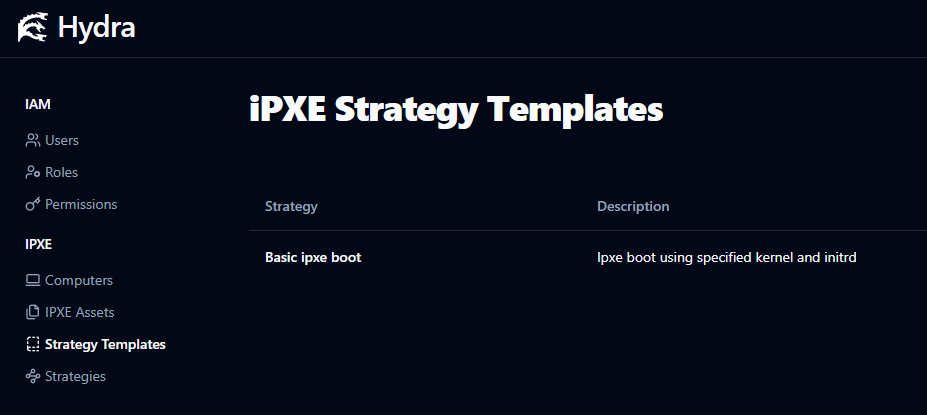
\includegraphics[width=\textwidth]{ipxe/startegy-templates.png}
  \caption{Strategy templates page}
\end{figure}

\subsection{Boot strategies}

Boot strategies can be thought of an instance of a strategy template that provides the data for the template to render.
They are created and managed on the \texttt{Strategies} page.
Each strategy template defines a different form that is used to create a new strategy.

\begin{figure}[H]
  \centering
  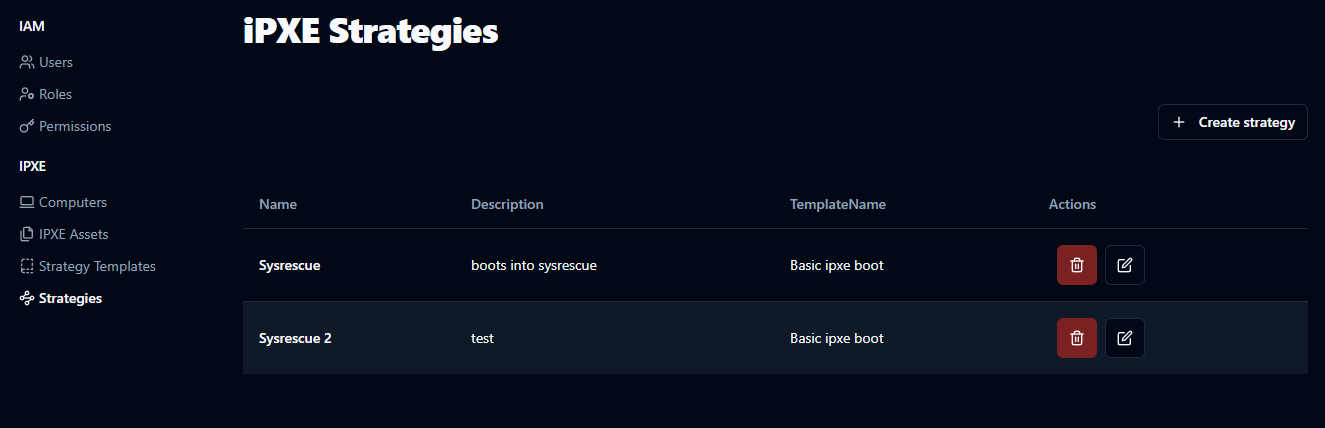
\includegraphics[width=\textwidth]{ipxe/strategies-page.png}
  \caption{View of existing boot strategies on the \texttt{Strategies} page}
\end{figure}

\begin{figure}[H]
  \centering
  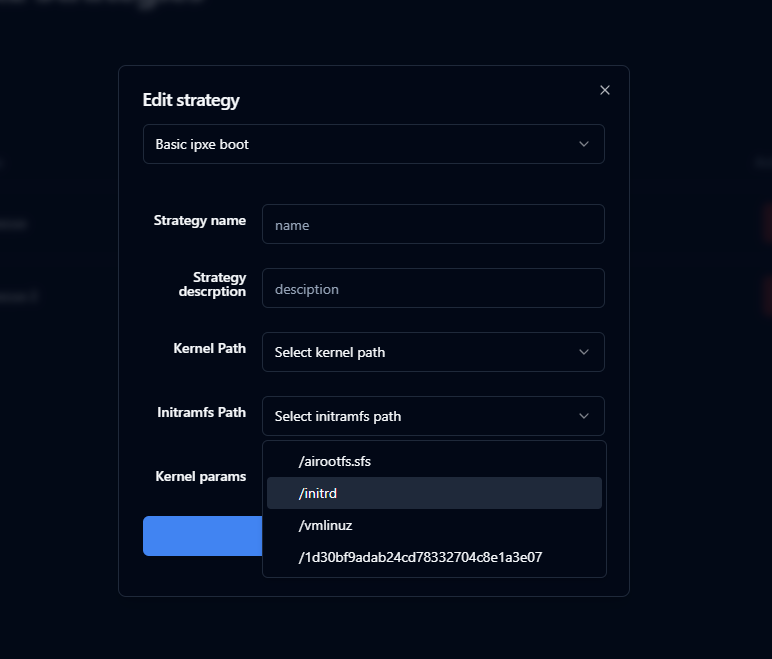
\includegraphics[width=0.8\textwidth]{ipxe/creating-new-boot-strategy.png}
  \caption{Creating a new boot strategy using basic boot template}
\end{figure}

\subsection{Selecting boot strategy}

Boot strategies are selected on the computers page. These strategies are set for each computer individually and can be changed at any time.
Computer groups can also have a boot strategy defined which is then used for all computers in the group that do not have a strategy selected.
Additionally, a global boot strategy can be selected which is used for all computers that do not have a strategy selected and are not in a group with a boot strategy selected.

\begin{figure}[H]
  \centering
  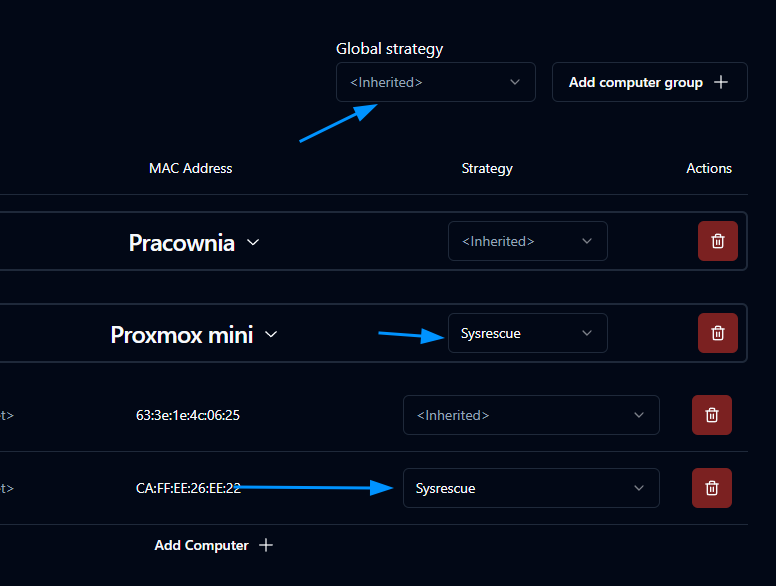
\includegraphics[width=0.8\textwidth]{ipxe/selecting-strategy.png}
  \caption{Selecting a boot strategy for a computer}
\end{figure}

\subsection{Requesting iPXE script}

Computers access the iPXE scripts by sending a HTTP request to the \texttt{/api/ipxe/boot/:mac} endpoint where \texttt{:mac} is the MAC address of the computer.
This is accomplished thanks to the embedded iPXE script that is included in the build firmware image. This script is shown in listing \ref{lst:ipxe-script}.

\begin{listing}[H]
  \textfile{implementation/code/ipxe/embedded-script.ipxe}
  \caption{Embedded iPXE script}
  \label{lst:ipxe-script}
\end{listing}

Swagger interface located at \texttt{api/docs} can be used to test the endpoint. Figure \ref{fig:request-example} shows an example request made to the endpoint using the MAC address
of one of the computers defined in the system.

\begin{figure}[H]
  \centering
  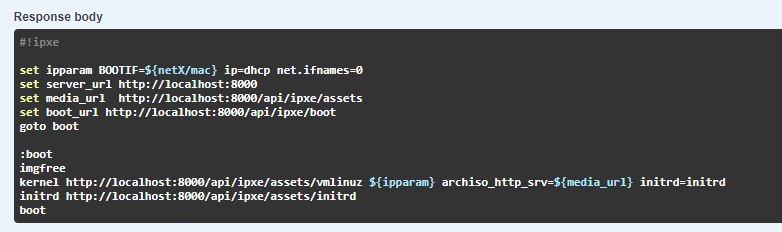
\includegraphics[width=\textwidth]{ipxe/example-response.png}
  \caption{Example request made to the \texttt{/api/ipxe/boot/:mac} endpoint}
  \label{fig:request-example}
\end{figure}

\subsection{iPXE exception filter}

When developing APIs it is a common practice to use exception to set the HTTP status code and message of the response.
This conversion from exception instance to HTTP response is handled by the \texttt{ExceptionFilter} class.

Nest already comes with a built-in exception filter that converts exceptions to HTTP responses.
This filter generates JSON responses that contain the exception message and the HTTP status code.
This is suitable for most APIs but not for the iPXE script endpoint as its consumers are expecting executable iPXE script and not a JSON response.
Failing to provide a valid iPXE script will result in the computer being stuck in an infinite boot loop which is not desirable.

For this purpose a custom exception filter was created that converts exceptions to executable iPXE scripts.
These script pause the boot process and display an appropriate error message.
Example of which is show in figure \ref{fig:exception-handling} when requesting a script for a computer that is not defined in the system.

\begin{figure}[H]
  \centering
  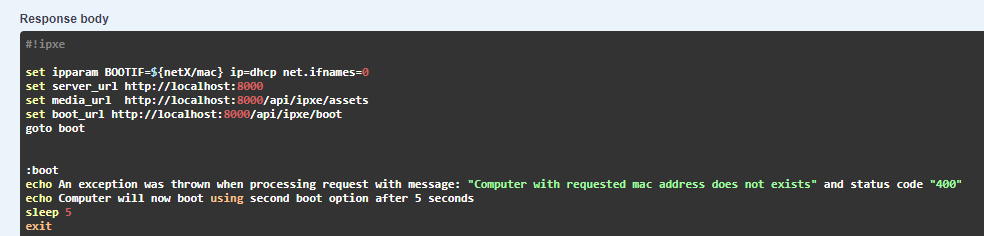
\includegraphics[width=\textwidth]{ipxe/exception-filter.png}
  \caption{Exception filter generated iPXE script}
  \label{fig:exception-handling}
\end{figure}

\end{document}